
%% INTRODUCTION %% 

\chapter{Introduction}
The current problem is described in the introduction, from which the motivation behind the bachelor thesis emerges. Subsequently, the goals that are pursued with the work are described.

\section{The Bachelor's Thesis Problem}
People in Germany are becoming more interested in physical and mental health matters. This is most likely attributed to the COVID-19 pandemic that has been circulating in recent years. \cite{.bahn-bonn} Along with positive outcomes, such as increased care for fellow citizens \cite{.bahn-bonn} and greater awareness of health issues, the consistent growth of interest in health issues also is causing problems. With an increasing number of anxious and concerned patients, medical practices and general practitioners have long since exceeded their capacity limits and have reached their breaking point \cite{.sok}. Patients also notice this: Overcrowded waiting rooms, long waiting periods, and nerve-racking telephone loops are becoming the norm for doctor visits. The BÄK (Bundesärztekammer), German Medical Association, draws attention to a second issue: as society ages, so does the medical industry. Every fifth doctor is about to retire. More than 13\% of doctors are between the ages of 60 and 65, while another 8.5\% are over the age of 65. Over the following few years, this will exacerbate clinics' and offices' already stressful staffing situation \cite{.blatt}. 
The bachelor`s thesis problem can be traced back to the preceding situation. The population is fearful, mainly caused by the COVID-19 pandemic, and doctors are reaching their limits. The resulting problems are of great importance. General practitioners are forced to order patient stops and issue access bans \cite{.sok}. This also means that patients needing immediate medical attention may be turned away, and medical care may be denied. In addition to the concerned patients, the number of seriously (COVID-19) ill people has steadily increased. There have been approximately 146,000 deaths in Germany since the start of the pandemic (as of August 19, 2022). \cite{.rki} As part of this work, a survey was launched to highlight the problem in more detail. The results indicate that around 80\% of those questioned have put off a visit to the doctor in recent years, even though they have suffered from symptoms.
\begin{figure}[H]
	\centering
	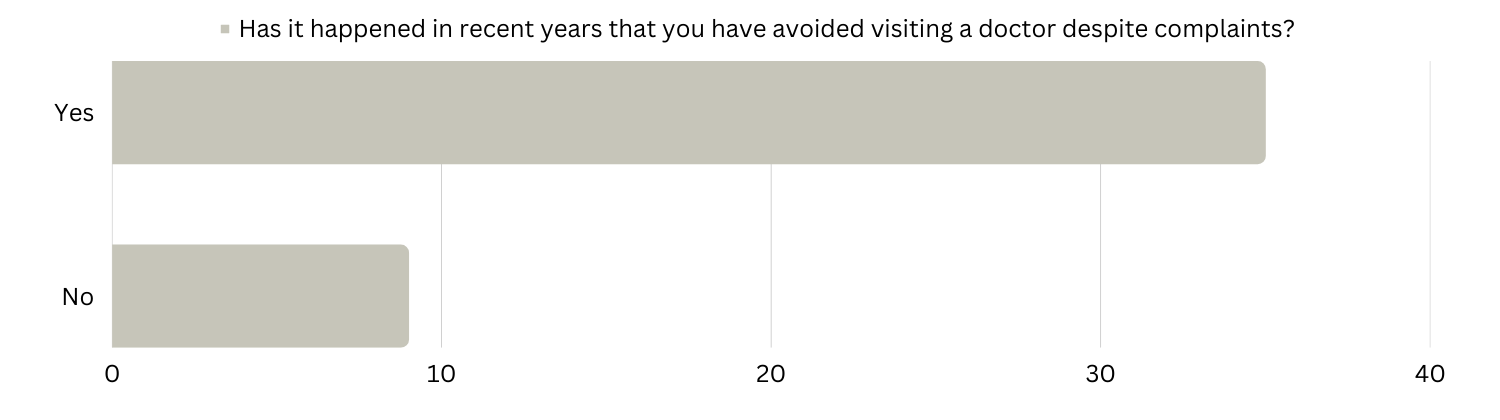
\includegraphics[scale=0.3]{avoidingDoctorYesNo.png}
	\caption[Survey Question]{Survey Question - Avoiding to visit the doctor}
\end{figure}
\noindent 
Another question in this survey asked respondents to list the justifications for delaying these doctor visits or the reasons they might consider forgoing a visit to the doctor. Those reasons range from long waiting times to difficulties scheduling an appointment. Figure 1.2 shows the mentioned distribution of the answers.
\begin{figure}[H]
	\centering
	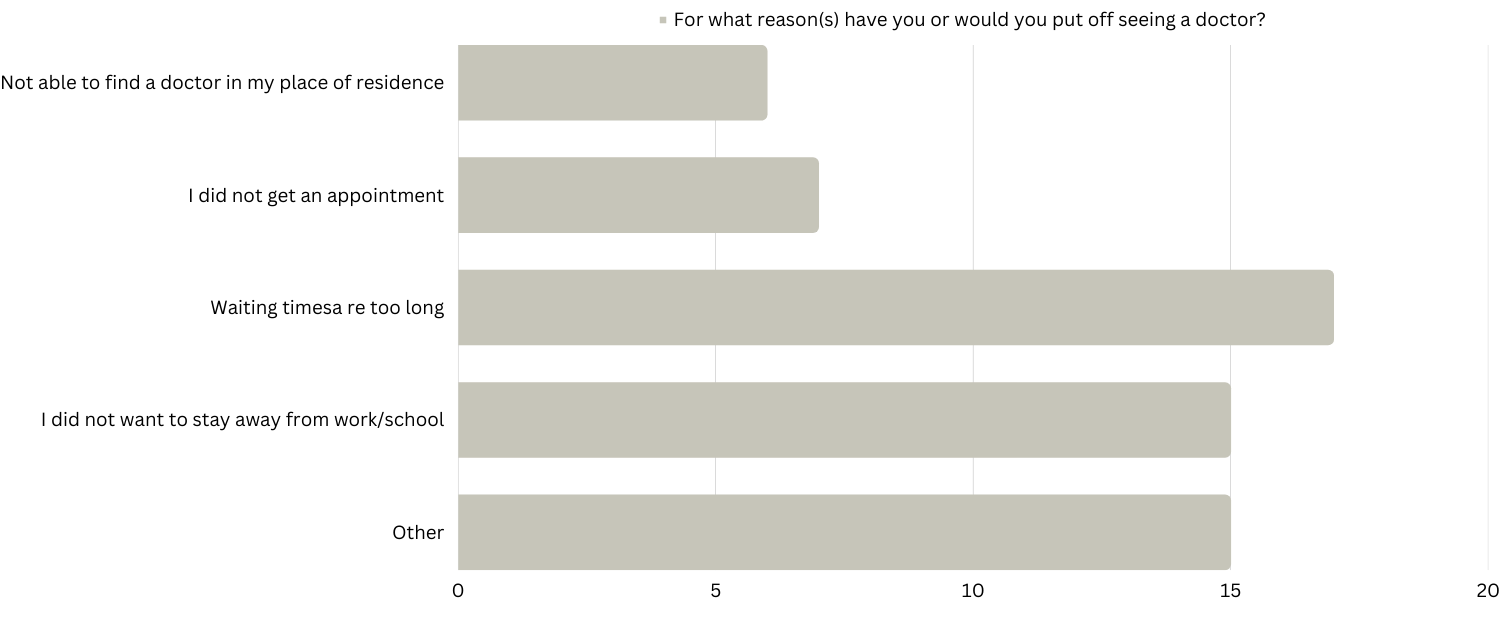
\includegraphics[scale=0.4]{reasonsPuttingOf.png}
	\caption[Survey Question]{Survey Question - Reasons of avoiding to visit the doctor}
\end{figure}
\noindent 
All questions of the survey, together with the answers, can be found in appendix A.
\section{Motivation}
The mentioned problem imposes the question of addressing patients’ concerns while relieving the burden on doctors. Digitalization provides a solution to this problem. Online consultation hours and appointment scheduling have recently helped relieve medical practices. Smartphones, in particular, are becoming an increasingly important part of our daily lives. The goal of this bachelor thesis is to provide a method for efficiently minimizing the problems mentioned above through the use of mobile applications. Such an application can advise a worried user and help alleviate their fears.

\section{The Bachelor Thesis Goal}
The goals of the bachelor thesis can be defined as follows:
\begin{itemize}
	\item Requirements analysis for the application
	\item Design and conception of the application
	\item Creation of a firestore database
	\item Comparing different algorithmic disease assignment methods
\end{itemize}
The application should be able to generate a diagnosis based on a user's specified symptoms. This diagnosis is made after successful data gathering regarding the user's symptoms and a subsequent determination of the possible diseases. Another goal of the application is that doctors can expand the database, whereby a verification possibility must be provided to ensure that the person trying to log in is, in fact, a doctor. They should be provided with the possibility to add disease-related data or advice regarding diseases and illnesses for users. In general, this is to create a place for users to get information regarding their health status and, at the same time, get advice on how to improve it.

\chapter{Related Works}
This chapter provides an overview of a selection of mobile applications comparable to the one in this work.

\section{Mobile Applications}
\subsubsection{ADA} 
\textbf{ADA} is the most prevalent symptom-detection smartphone application. According to their statements, their users are currently around 12 million, while 28 million symptom analyses have already been completed \cite{.adaHOME}. The application is free in the PlayStore and the Apple Store. Disease detection in the ADA application is based on AI (Artificial Intelligence) developed by medical professionals of the ADA team. The user can provide personal data in their user profile, such as allergies and medication intake. A symptom analysis starts by asking the user what their worst symptom is. Based on the user's answer, the AI searches its medical lexicon for this symptom and asks a symptom-specific question.
An example of this would be to ask the user if he had enough water today for the symptom headache. ADA uses a specially developed reasoning technology to assign symptoms. For this purpose, each symptom and each disease was assigned a joint probability, which makes it possible to calculate the overall probability of the disease for the specific symptom analysis \cite{.adaKI}. After the successful diagnosis, the user can download the diagnosis in PDF format, while they are also saved internally. The ADA application also makes its collection of knowledge available to users in the form of a disease dictionary. ADA also offers an API (Application Programming Interface), which enables healthcare organizations to integrate the AI chatbot into their application with the help of platform-specific SDKs (Software Development Kits)\cite{.adaFAQ} \cite{.adaDOCU}.

\subsubsection{Symptom Checker} 
The \textbf{Symptom Checker} is another currently available application. It was created using the computer language C\# and the Unity platform \cite{.symptomchecker}. Here, the user can select from a list of disease specifications, including those for diabetes tests, thrombosis, depression, hair loss, headache, and gastrointestinal infection. During the survey procedure, a doctor's interview is simulated, where the user is prompted with questions after choosing one of these categories, similar to the ADA application. The most likely condition is then diagnosed based on the patient's responses, and various treatment choices are provided. The application was made specifically for people without medical experience and was created by German doctors and medical experts. According to the developers, an algorithm that accesses a medical database produces the diagnosis \cite{.symptomchecker}. Sadly, nothing more can be found about the algorithm and how it works. 

\subsubsection{Other Solutions}
In addition to ADA and the Symptom Checker, other applications for symptom detection are available in the Play Store. However, these are less accurate than those mentioned. Some of these applications are only intended as a reference book for symptoms and diseases without a disease determination. In addition to mobile applications, some web applications and websites are available. However, this will not be discussed further in this work since only mobile applications are dealt with here.

\section{Differentiation from other Systems}
In contrast to both of the applications mentioned, the system's knowledge base should be expanded by doctors who are not part of the development team. Similar to the Diagnosis App, the application presented in this work will not request any personally identifiable information from users. An exception is a case when users wish to identify themselves as doctors. Unlike ADA, the diagnoses are not generated using AI but are calculated by an algorithm. As already mentioned, the calculation process of the Diagnosis app cannot be determined, and therefore no differentiation can be made from this application. With a realistic view, this application cannot work as accurately as artificial intelligence, which has been trained since 2011. This work should not replace ADA as the market leader, not the Diagnosis App, but describe the possible conception and implementation of such an application while comparing different calculation possibilities of the possible diseases based on the user symptoms.




